\documentclass[12pt]{article}

% Packages
\usepackage[margin=0.6in]{geometry}
\usepackage{graphicx}
\usepackage{amsmath}
\usepackage{float}
\usepackage[dvipsnames]{xcolor}
\usepackage{etoolbox}
\usepackage{soul}
\usepackage{amsbsy}

\pagestyle{plain}


\begin{document}

\title{Solution ark \#7.\\ Variance estimation}
\author{O\u{g}uz--Alper, Melike \& Pekarskaya, Tatsiana, Statistics Norway}
\maketitle

\section*{Exercise 1}
\textbf{\color{ForestGreen}(R code available)} Use the data in srs30.dat, which includes $n=30$ units selected with simple random sampling from an artificial population of size $N=100$. 
\begin{enumerate}
\item Use the jackknife to estimate $V(\bar{y})$, and verify that $\hat{V}_{JK}(\bar{y})=s^2/30$ for this data. What are the jackknife weights for jackknife replicate $j$? \\
\fcolorbox{black}{ForestGreen!20}{
\begin{minipage}[t]{0.97\linewidth}
\textbf{Solution:}

As SRS of size $n=30$ from an artificial population of size $N=100$. \textbf{a.} Use the jackknife to estimate $V(\bar{y})$ for srs30.dat. 
The customary jackknife estimator is given by
$$\hat{V}_{JK}(\bar{y})=\frac{n-1}{n}\sum_{j \in s}\Big(\bar{y}_{-j}-\frac{1}{n}\sum_{j \in s}\bar{y}_{-j}\Big)^2, \quad \bar{y}_{-j}=\sum_{i \in s}w_{i(j)} y_i/N,$$
where $w_{i(j)}$ are the jackknife weights for jackknife replicate $j$:
\begin{eqnarray*}
w_{i(j)}=\left\{
\begin{array}{lcl}
0 & \text{if} & i=j \\
\frac{30}{29}w_i &\text{if} & i\neq j
\end{array}
\right.\cdot
\end{eqnarray*}
We have $w_i=100/30$ under SRS. Hence, $w_{i(j)}=(30/29)(100/30)=3.44828$ for $i\neq j$.
We have $\bar{y}_{-j}=\sum_{i\neq j \in s} y_i/(n-1)$, as $w_{i(j)}=N/(n-1)$ for $i\neq j$, and 
$$\frac{1}{n}\sum_{j \in s}\bar{y}_{-j}=\frac{1}{n}\frac{1}{n-1}\sum_{j \in s}\sum_{i\neq j \in s} y_i=\frac{1}{n}\frac{1}{n-1}\sum_{j \in s}(n-1)y_j=\bar{y}\cdot$$
$\bar{y}_{-j}$ can be can re-written as follows.
$$\bar{y}_{-j}=\frac{1}{n-1}\Big(\sum_{i \in s}y_i-y_j\Big)=\frac{1}{n-1}(n\bar{y}-y_j)=\bar{y}-\frac{1}{n-1}(y_j-\bar{y})\cdot$$
Thus we have
$$\hat{V}_{JK}(\bar{y})=\frac{n-1}{n}\frac{1}{(n-1)^2}\sum_{j \in s}(y_j-\bar{y})^2=\frac{s_y^2}{n}\cdot$$
\end{minipage}}\\
\fcolorbox{black}{ForestGreen!20}{
\begin{minipage}[t]{0.97\linewidth}
For this data, we have $\bar{y}= 8.233333$, and $\bar{y}_{-1}=8.241379,\, \bar{y}_{-2}=8.344828,\cdots,\bar{y}_{-30}=8.206897$.
$$\hat{V}_{JK}(\bar{y})=\frac{30}{29}0.5509711=0.5326054,$$
$${s_y^2}/{30}={15.97816}/{30}=0.5326054\cdot$$
Using the finite population correction, we obtain
$$\Big(1-\frac{n}{N}\Big)\hat{V}_{JK}(\bar{y})=\Big(1-\frac{30}{100}\Big)0.5326054=0.3728238\cdot$$

\end{minipage}}
\item Find also the bootstrap estimate of $V(\bar{y})$. \\
\fcolorbox{black}{ForestGreen!20}{
\begin{minipage}[t]{0.97\linewidth}
\textbf{Solution:}
An estimate of the population mean $\bar{y}$ at the $b$th bootstrap replicate is found by, respectively with the naive bootstrap and the rescaling bootstrap with $m=n-1$
$$\bar{y}_{r,MC}^{*}=\frac{\sum_{i \in s} \tau_{ri}y_i }{n} ,\quad\bar{y}_{r}^{*}=\frac{\sum_{i \in s}w_{ri}^{*} y_i}{\sum_{i \in s}w_{ri}^{*}},\quad w_{ri}^{*} =\tau_{ri}^{*}\left(\frac{n}{n-1}\right)\left(\frac{N}{n}\right)\cdot$$
Here, $\bar{y}_{r,MC}^{*}=\bar{y}_{r}^{*}$, as the rescaling bootstrap with $m=n-1$ reduces to the naive bootstrap with replicates of size of $n-1$.
$$\hat{V}_{boot}(\bar{y})=\frac{1}{R-1}\sum_{r=1}^R\left(\bar{y}_{r}^{*}-\frac{1}{R}\sum_{r=1}^R\bar{y}_{r}^{*}\right)^2\cdot$$
\begin{figure}[H]
\begin{center}
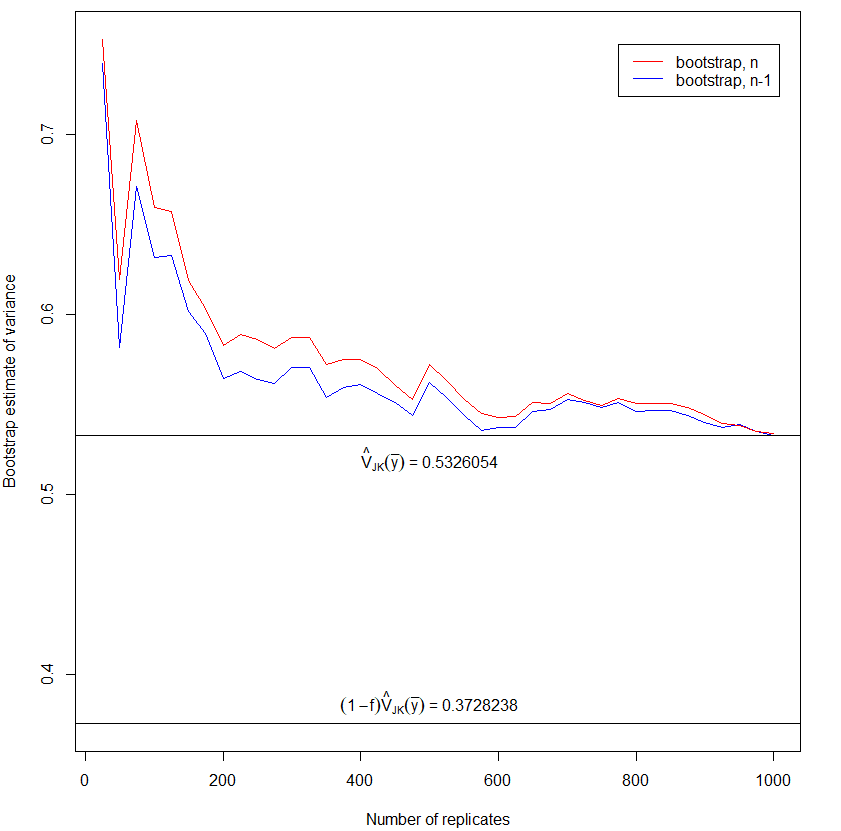
\includegraphics[scale=0.55]{Ex1_2.png}
\end{center}
\end{figure}
\end{minipage}}
\end{enumerate}

\section*{Exercise 2}
\textbf{\color{ForestGreen}(R code available)} The file agsrs.dat contains data from an SRS of $300$ of the $3\,078$ counties.
Let $y_i$ be total acreage of farms in county $i$ in 1992 and $x_i$ be total acreage of farms in county $i$ in 1987. Use the jackknife and the bootstrap to estimate the variance of the ratio estimator $\hat{B}_r=\bar{y}/\bar{x}$. How do they compare with the linearization estimator? \\
\fcolorbox{black}{ForestGreen!20}{
\begin{minipage}[t]{0.97\linewidth}
\textbf{Solution:}

An SRS of $n=300$ of the $N=3\,078$ counties.
$y_i$: total acreage of farms in county $i$ in 1992; $x_i$: total acreage of farms in county $i$ in 1987. Estimate $V(\hat{B})$ with $\hat{B}=\bar{y}/\bar{x}$ using the resampling methods. \\
We have $$\hat{B}=297\,897/301\,953.7= 0.9865652\cdot$$
For the jackknife, we have
$$\hat{B}_{-j}=\frac{\bar{y}_{-j}}{\bar{x}_{-j}},\quad \bar{y}_{-j}=\frac{1}{n-1}\sum_{i\neq j\in s}y_i,\;\bar{x}_{-j}=\frac{1}{n-1}\sum_{i\neq j\in s}x_i,$$
$$\frac{1}{n}\sum_{j \in s}\hat{B}_{-j}=0.9865651\cdot$$

The jackknife variance estimator provides
$$\hat{V}_{JK}(\hat{B})=\frac{299}{300}\sum_{j\in s}\Big(\hat{B}_{-j}-0.9865651\Big)^2=3.707\times10^{-05},$$
$$\Big(1-\frac{300}{3\,078}\Big)\hat{V}_{JK}(\hat{B})=3.346\times10^{-05}\cdot$$
The ratio estimate at the $r$th bootstrap replicate is found by
$$\hat{B}_{r}^*=\frac{\bar{y}_{r}^*}{\bar{x}_{r}^*},\quad \bar{y}_{r}^*=\frac{\sum_{i\in s}\tau_{ri} y_i}{m}, \; \bar{x}_{r}^*=\frac{\sum_{i\in s}\tau_{ri} x_i}{m}, \quad m=n, n-1\cdot$$
$$\hat{V}_{boot}(\hat{B})=\frac{1}{R-1}\sum_{r=1}^R\left(\hat{B}_{r}^*-\frac{1}{R}\sum_{r=1}^R\hat{B}_{r}^*\right)^2\cdot$$

The variance estimator with the linearization method, 
$$\hat{V}_L(\hat{B})=(1-f)\frac{1}{\bar{x}^2}\frac{s_e^2}{n},$$
where
$$s_e^2=\frac{1}{n-1}\sum_{i\in s}(e_i-\bar{e})^2, \quad e_i=y_i-\hat{B} x_i,$$ 
provides
$$\hat{V}_L(\hat{B})=\Big(1-\frac{300}{3\,078}\Big)\frac{1}{(301\,953.7)^2}\frac{1\,002\,179\,462}{300}=3.307\times 10^{-05}\cdot$$
\end{minipage}}\\
\fcolorbox{black}{ForestGreen!20}{
\begin{minipage}[t]{0.97\linewidth}

\begin{figure}[H]
\begin{center}
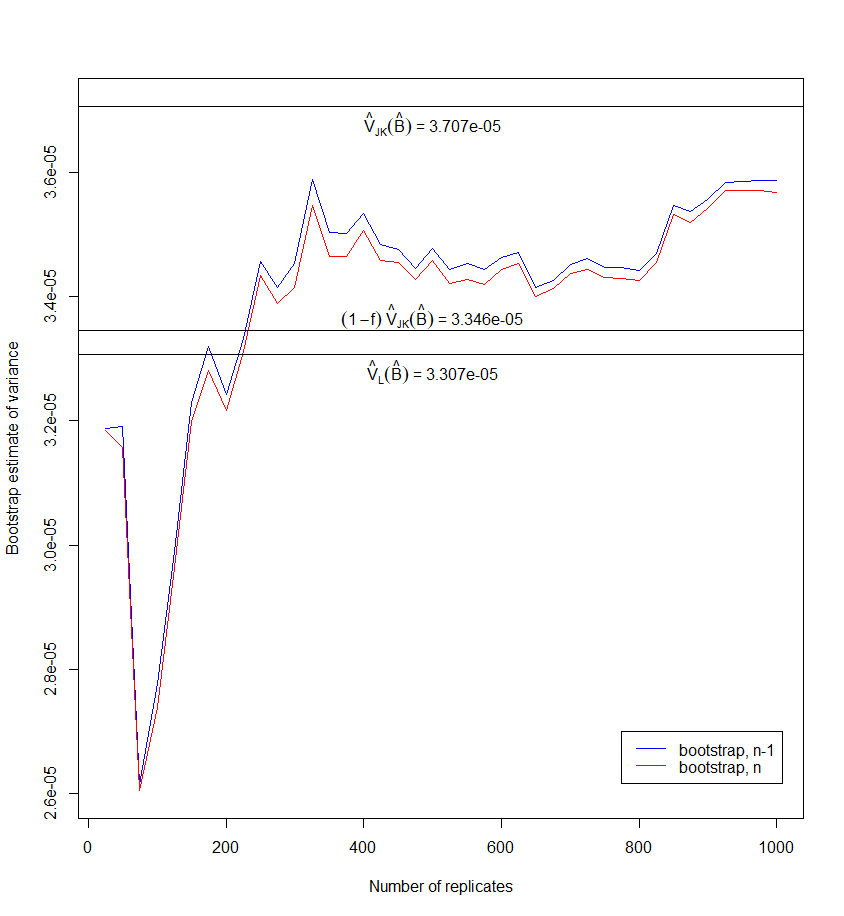
\includegraphics[scale=0.55]{Ex2.png}
\end{center}
\end{figure}

\end{minipage}}


\section*{Exercise 3}
\textbf{\color{ForestGreen}(R code available)} Foresters want to estimate the average age of trees in a stand. Determining age is
cumbersome, because one needs to count the tree rings on a core taken from the
tree. In general, though, the older the tree, the larger the diameter, and diameter
is easy to measure. The foresters measure the diameter of all $1\,132$ trees and find
that the population mean equals $10.3$. They then randomly select $20$ trees for age
measurement.
\begin{center}
\begin{tabular}{rrrrrr}
Tree No. & Diameter, $x$ & Age, $y$& Tree No.& Diameter, $x$ &Age, $y$ \\
\hline
1& 12.0& 125 &11 &5.7 &61\\
2& 11.4& 119 &12& 8.0 &80\\
3& 7.9 &83 &13 &10.3& 114\\
4& 9.0 &85& 14 &12.0& 147\\
5& 10.5& 99& 15 &9.2 &122\\
6& 7.9 &117& 16 &8.5& 106\\
7& 7.3& 69 &17 &7.0& 82\\
8& 10.2& 133& 18& 10.7 &88\\
9& 11.7& 154 &19 &9.3 &97\\
10& 11.3& 168 &20& 8.2& 99\\
\end{tabular}
\end{center}
Using the jackknife and the bootstrap, estimate the standard error for the regression estimate of the
population age of trees in a stand. How
do the jackknife and bootstrap compare with the standard error calculated using linearization
methods? \\
\fcolorbox{black}{ForestGreen!20}{
\begin{minipage}[t]{0.97\linewidth}
\textbf{Solution:}

Survey of trees, SRS. $N=1\,132$ and $n=20$. $y_i$: age of the $i$th tree: $x_i$: the diameter of the $i$th tree. The population average: $\bar{x}=10.3$. Estimate $V(\bar{y}_{reg})$ using the resampling methods.\\
We have
$$\hat{B}_1=\frac{\sum_{i\in s}(x_i-\bar{x})(y_i-\bar{y})}{\sum_{i\in s}(x_i-\bar{x})^2}=12.24966,$$
$$\hat{B}_0=\bar{y}-\hat{B}_1\bar{x}=107.4-12.24966(9.405)=-7.808087,$$
$$\bar{y}_{reg}=\hat{B}_0+\hat{B}_1\bar{X}=-7.808087+12.24966(10.3)=118.3634\cdot$$
For the jackknife, we have
$$\bar{y}_{reg, (j)}=\hat{B}_{0 (j)}+\hat{B}_{1 (j)}\bar{X},$$
$$\hat{B}_{0 (j)}=\bar{y}_{-j}-\hat{B}_{1 (j)}\bar{x}_{-j},\quad \hat{B}_{1 (j)}=\frac{\sum_{i\neq j\in s}(x_i-\bar{x}_{-j})(y_i-\bar{y}_{-j})}{\sum_{i\neq j\in s}(x_i-\bar{x}_{-j})^2}\cdot$$
$$\frac{1}{n}\sum_{j \in s}\bar{y}_{reg (j)}=118.3579\cdot$$
$$\widehat{SE}_{JK}(\bar{y}_{reg})=\sqrt{\frac{19}{20}\sum_{j\in s}(\bar{y}_{reg(j)}-118.3579)^2}=5.384611\cdot$$
$$\sqrt{1-\frac{20}{1\,103}}\widehat{SE}_{JK}(\bar{y}_{reg})=0.9911267(5.384611)=5.336832\cdot$$
The regression estimate of the mean at the $r$th bootstrap replicate is given by
$$\bar{y}_{reg(r)}^*=\hat{B}_{0(r)}^*-\hat{B}_{1(r)}^*\bar{x},$$
$$\hat{B}_{0(r)}^*=\bar{y}_r-\hat{B}_{1(r)}^*\bar{x}_r,$$
$$\hat{B}_{1(r)}^*=\frac{\sum_{i\in s}\tau_{ri}(x_i-\bar{x}_r)(y_i-\bar{y}_r)}{\sum_{i\in s}\tau_{ri}(x_i-\bar{x}_r)^2}\cdot$$
$$\widehat{SE}_{boot}(\bar{y}_{reg})=\sqrt{\frac{1}{R-1}\sum_{r=1}^R\left(\bar{y}_{reg(r)}^*-\frac{1}{R}\sum_{r=1}^B\bar{y}_{reg(r)}^*\right)^2}\cdot$$
The linearization variance estimator provides
$$\widehat{SE}_L(\bar{y}_{reg})=\sqrt{\Big(1-\frac{20}{1\,132}\Big)\frac{s_e^2}{20}}=\sqrt{\Big(1-\frac{20}{1\,132}\Big)\frac{319.6277
}{20}}=3.9622,$$
where $s_e^2$ is the sample variance of $e_i=y_i-\hat{B}_0-\hat{B}_1  x_i$.
\end{minipage}}\\
\fcolorbox{black}{ForestGreen!20}{
\begin{minipage}[t]{0.97\linewidth}
The alternative linearization estimator of the variance (Lohr 2019, p. 459), which is also the one used by the \emph{survey} R package, provides
$$\widehat{SE}_{Lalt}(\bar{y}_{reg})=\sqrt{\hat{V}\Big(\sum_{i\in s}w_ig_ie_i\Big)}=5.065371, \quad w_i=N/n,$$
where $g_i=1+(\boldsymbol{t_x}-\boldsymbol{\hat{t}_x})^\top\left(\sum_{i\in s}w_i\boldsymbol{x_i}\boldsymbol{x_i}^\top\right)^{-1}\boldsymbol{x_i}$, with $\boldsymbol{t_x}=(N,X)^\top$, $\boldsymbol{\hat{x}_x}=(\hat{N},\hat{X})^\top$, and $\boldsymbol{x_i}=(1,x_i)^\top$.
\begin{figure}[H]
\begin{center}
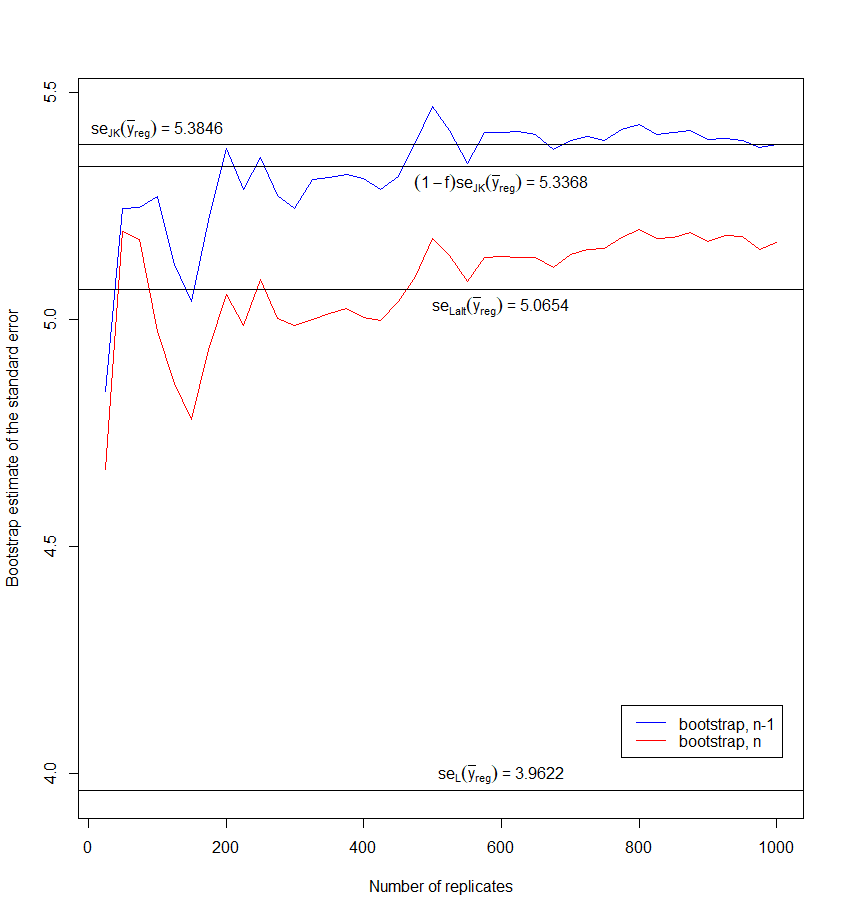
\includegraphics[scale=0.55]{Ex3.png}
\end{center}
\end{figure}

\end{minipage}}

\section*{Exercise 4}
\textbf{\color{ForestGreen}(R code available)} The American Statistical Association (ASA) studied whether it should offer a certification
designation for its members, so that statisticians meeting the qualifications
could be designated as “Certified Statisticians.” In 1994, the ASA surveyed its membership
about this issue, with data in file certify.dat. The survey was sent to all 18 609
members; 5 001 responses were obtained. Results from the survey were reported in the October 1994 issue of Amstat News.\\
Assume that in 1994, the ASA membership had the following characteristics: $55\%$
have PhD’s and $38\%$ have Master’s degrees; $29\%$ work in industry, $34\%$ work in
academia, and $11\%$ work in government. The cross-classification between education
and workplace was unavailable. There is a nonresponse. However, treat as if the respondents were selected with a probability sampling from the list of all members. Find the raking estimate of the total number of ASA members for this exercise. Estimate the total number of members opposing certification in 1994 using and use the bootstrap to estimate its variance and construct a $95\%$ confidence interval.\\
\fcolorbox{black}{ForestGreen!20}{
\begin{minipage}[t]{0.97\linewidth}
\textbf{Solution:}

ASA survey of certification designation for its members. $n=N=18\,609$ and $n=5\,001$. Treat respondents as the sample selected from the list of members.\\
Sample distribution by education and workplace is given as follows:
\begin{center}
\begin{tabular}{lrrrrr}
&Industry & Academia& Other&\vline & \\
\hline
PhD& 798& 1 787& 451& \vline &3 036\\
non-PhD& 1 011& 434 &520& \vline &1 965\\
\hline
&1 809 &2 221& 971&\vline & 5 001 \\
\end{tabular}
\end{center}  
Only the marginal totals are known in the population. Using the raking weights, we obtain 
\vspace{-0.3 cm}
$$\hat{Y}_{rak}=\sum_{i \in s}w_{i(rak)}y_i=7\,313.734,$$
\vspace{-0.3 cm}\\
where $y_i=1$ if member $i$ opposes certification and zero otherwise.
There is no analytical expression for the iterative raking. For each bootstrap replication, raking is applied to the subsample selected. Initial weights are set to $w_{0ri}^*=w_in/m$, where $w_i=18\,806/5\,001=3.721056$ and $m$ is the subsample size. Raking weights are then used to find the bootstrap estimates.\\
With $R=1000$ and $m=n-1$, we obtain
\vspace{-0.3 cm}
$$\frac{1}{1000}\sum_{r=1}^{1000}\hat{Y}_{rak(r)}^*=7\,315.3,$$
\vspace{-0.3 cm}
$$\hat{V}_{boot}(\hat{Y}_{rak})=\frac{1}{999}\sum_{r=1}^{1000}(\hat{Y}_{rak(r)}^*-7\,315.3)^2=19\,196.81\cdot$$
\vspace{-0.5 cm}
\begin{figure}[H]
\begin{center}
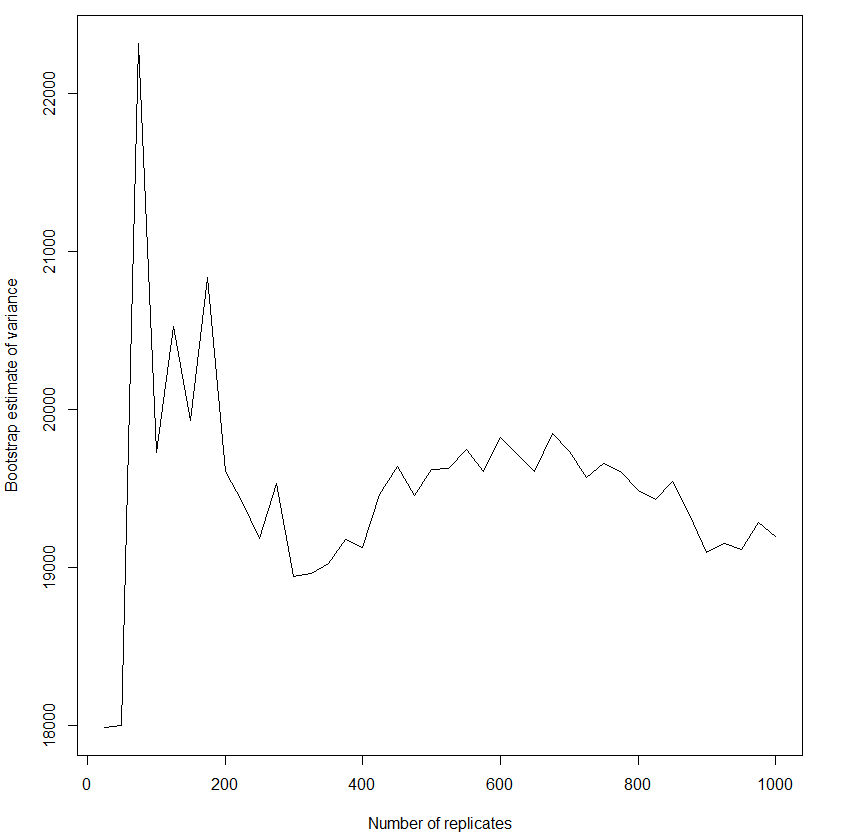
\includegraphics[scale=0.5]{Ex4.png}
\end{center}
\end{figure}

\end{minipage}}\\
\fcolorbox{black}{ForestGreen!20}{
\begin{minipage}[t]{0.97\linewidth}
The standard $95\%$ CI is given by
$$7\,313.734\pm 1.96\sqrt{19\,196.81}=[7\,042.176,7\,134.180]$$
The $95\%$ CI obtained from the $2.5$th and the $97.5$th percentiles of the distribution of the bootstrap estimates $\hat{Y}_{rak(r)}^*$ is given as follows.
$$[7\,040.938,7\,133.355]\cdot$$
\begin{itemize}
\item Both methods provide similar bounds.
\item The sample size is very large, making the normality assumption reasonable. 
\end{itemize}
\end{minipage}}

\end{document}